% MEDSYS paper draft: IEEE conference format, 6-page limit INCLUDING references.
% Compile (Overleaf or TeX Live): pdflatex medsys-paper; bibtex medsys-paper; pdflatex x2.
%
% Open items before submission (kept here, not in the PDF, to save space):
%  1. Affiliations and e-mails (authors: Sameer Morya, Sarthak Wage), acknowledgements.
%  2. Logged systematic literature search (Phase 0) to confirm the novelty claim in Sec. I-II;
%     read the full texts of Juergensen et al. and Ahmed et al. (segmentation methods used).
%  3. CT-ORG (liver; lungs and bone in cases 0-20) as a held-out multi-organ set.
%  4. Median [IQR] and worst case, NSD at 0.5/1/2 mm, mixed-effects attribution.
%  5. Local error heatmaps; 3D Slicer meshing baseline on identical masks.
%  6. Check the page count after every edit: the limit is 6 pages including references.
%
% Title options (12-18 words): A (used) Stage-Wise Attribution of Geometric Error in Automatic
% Anatomical Surface Reconstruction From Computed Tomography; B Resolution, Segmentation or
% Smoothing? Attributing Surface Error in Automatic Reconstruction of Anatomy From Computed Tomography.
\documentclass[conference]{IEEEtran}

\usepackage{cite}
\usepackage{amsmath,amssymb}
\usepackage{graphicx}
\usepackage{booktabs}
\usepackage{array}
\usepackage{xcolor}
\usepackage{url}
\usepackage{xspace}
\usepackage{iftex}
% IEEEtran sets Times for pdfLaTeX. Under XeLaTeX (e.g. Tectonic) Times is not found that way,
% so load TeX Gyre Termes, a metric-compatible Times clone, to keep the same layout and length.
\ifXeTeX
  \usepackage{fontspec}
  \setmainfont{texgyretermes}[Extension=.otf, UprightFont=*-regular, BoldFont=*-bold,
    ItalicFont=*-italic, BoldItalicFont=*-bolditalic]
\fi

\graphicspath{{figures/}}
\newcommand{\todo}[1]{\textcolor{red}{[TODO: #1]}}
\newcommand{\lvl}[1]{\texttt{#1}}
\newcommand{\mm}{\,mm\xspace}

\begin{document}

\title{Stage-Wise Attribution of Geometric Error in Automatic Anatomical Surface Reconstruction From Computed Tomography}

\author{\IEEEauthorblockN{Sameer Morya}
\IEEEauthorblockA{\todo{Dept., University, City}\\ \todo{e-mail}}
\and
\IEEEauthorblockN{Sarthak Wage}
\IEEEauthorblockA{\todo{Dept., University, City}\\ \todo{e-mail}}}

\maketitle

\begin{abstract}
Automatic pipelines turn computed tomography (CT) into surface models, but their geometric error is rarely traced to its source, and prior error budgets add stage errors measured one at a time. This study crosses resolution, segmentation and reconstruction in a factorial design against two references: four analytic phantoms with exact surfaces (7{,}760 meshes), and 41 expert-labelled spleen CT scans resampled before segmentation by TotalSegmentator (16{,}072 meshes). Across the tested grids, spacing had the largest descriptive share of error variance on exact surfaces (38.8\%) and on correct segmentations of real anatomy (50.5\%). Under simulated coarsening, error followed the empirical relationship $\text{ASSD}\approx0.177\,\Delta$ (95\% CI 0.171--0.184; leave-one-scan-out $R^2=0.75$), with $\Delta$ the sampling added, while Dice stayed at or above 0.968. For the engine, scans accounted for 89.5\% of the variance (94.2\% in a random-intercept model); its error was unchanged from native to 3\mm grids (0.901 and 0.907\mm) but rose by 0.188\mm with 5\mm slices. Decimation broke mesh closure without moving unsmoothed geometry, and meshing on the engine's 3\mm working grid improved closure at identical physical settings. On this dataset and engine, slice thickness and case difficulty dominate the error budget.
\end{abstract}

\begin{IEEEkeywords}
Marching cubes, mesh decimation, Taubin smoothing, surface distance, digital phantoms, slice thickness, segmentation evaluation, 3D printing.
\end{IEEEkeywords}

% ════════════════════════════════════════════════════════════════════════
\section{Introduction}
Surface models built from CT are now routine in surgical planning, teaching and 3D printing~\cite{schulze2024qa}, and engines such as TotalSegmentator~\cite{wasserthal2023totalsegmentator}, built on nnU-Net~\cite{isensee2021nnunet}, have made segmentation automatic. A pipeline still makes several decisions after segmentation: it extracts an isosurface~\cite{lorensen1987marching,lewiner2003marching}, smooths it~\cite{taubin1995signal} and simplifies it~\cite{schroeder1992decimation}. Each can move the surface, and the scan's resolution limits what any of them can recover.

Accuracy studies of such models come mainly from 3D printing, where total error is split into segmentation, digital editing and printing error~\cite{schulze2024qa}. Their methodology measures each stage separately, on one phantom or structure with threshold-based segmentation, and adds the partial errors~\cite{juergensen2024phantom}; automatic engines, meanwhile, are evaluated at mask level~\cite{antonelli2022msd,wasserthal2023totalsegmentator}, so the surface a user finally sees is rarely scored. Two methodological gaps follow: an additive error budget cannot represent interactions between stages, and without an exact reference the error of the reference itself cannot be separated from that of the pipeline.

This paper addresses the attribution of geometric error in \emph{automatic} pipelines, against both exact and expert references, through four questions. \textbf{Q1:} How much error does reconstruction itself introduce when the true surface is known, and which factor dominates? \textbf{Q2:} How far does coarser acquisition alone move the surface of a correct segmentation of real anatomy, and is the effect predictable? \textbf{Q3:} Does an automatic engine's surface error depend on resolution, and how is its variance shared between patient, resolution and reconstruction? \textbf{Q4:} How do the settings a deployed pipeline ships affect geometry and topology?

The contributions are methodological first: (1)~a two-reference factorial design that crosses all stages against exact and expert references, with resolution controlled before segmentation (Section~II); (2)~a scan-clustered attribution showing that spacing dominates error for correct segmentations but the patient dominates for an automatic engine; (3)~an empirical sampling relationship, $\text{ASSD}\approx0.177\,\Delta$, validated across scans, that predicts the error added by simulated coarsening and bounds useful metric tolerances; and (4)~practical findings on Dice, blur, decimation and meshing grids for deployed pipelines. The study makes no clinical claim, and its real-anatomy results cover one organ, one dataset and one engine mode. Sections~II--V give related work, definitions, the framework and the setup; Section~VI answers Q1--Q4; Sections~VII--X test, discuss, qualify and conclude.

% ════════════════════════════════════════════════════════════════════════
\section{Related Work}
\emph{Error decomposition in anatomical modelling.} Schulze \emph{et al.} reviewed 139 studies and organised their errors into segmentation, digital editing and printing error: the median segmentation error was 0.8\mm against 0.26\mm for printing, no average was found for digital editing, and the total did not exceed the partial errors, which may compensate each other~\cite{schulze2024qa}. Juergensen \emph{et al.} evaluated the three stages individually on one physical phantom, varying slice thickness, kernel, threshold, smoothing, software and printer, and computed the total error as their sum~\cite{juergensen2024phantom}. Ahmed \emph{et al.} crossed slice thickness and pixel size on six cadaver mandibles, scored against surface scans of the dissected bone, and found that slice thickness alone mattered~\cite{ahmed2024mandible}.

\emph{Reconstruction and evaluation.} Marching cubes~\cite{lorensen1987marching,lewiner2003marching}, Taubin smoothing~\cite{taubin1995signal} and decimation~\cite{schroeder1992decimation} are standard; smoothing trades staircase artefacts against shape and volume on medical surfaces~\cite{bade2006smoothing}, and simplification error is usually measured between a mesh and its own original~\cite{cignoni1998metro}, not against anatomy. Guidelines recommend boundary metrics alongside overlap~\cite{maierhein2024metrics,nikolov2021nsd}, yet benchmarks score masks, not meshes~\cite{antonelli2022msd}, and quality estimation without ground truth~\cite{valindria2017rca,wundram2024conformal} likewise stops at the mask.

\begin{table}[!t]
\caption{Design of the closest prior studies and of this work (prior designs as stated in their abstracts).}
\label{t:related}
\centering\scriptsize
\setlength{\tabcolsep}{3pt}
\begin{tabular}{@{}>{\raggedright\arraybackslash}p{1.45cm}>{\raggedright\arraybackslash}p{1.65cm}>{\raggedright\arraybackslash}p{1.35cm}>{\raggedright\arraybackslash}p{2.05cm}>{\raggedright\arraybackslash}p{1.15cm}@{}}
\toprule
Study & Reference & Segmentation & Design & Scale \\
\midrule
Juergensen~\cite{juergensen2024phantom} & 3D scan of a physical phantom & threshold & stages one at a time; total = sum & 1 phantom \\
Ahmed~\cite{ahmed2024mandible} & scan of dissected bone & not stated & slice $\times$ pixel size & 6 cadavers \\
Schulze~\cite{schulze2024qa} & (review) & various & categorised reported errors & 139 studies \\
This work & exact surfaces; expert masks & deep-learning engine; expert mask & full factorial; scan-clustered & 4 phantoms; 41 scans \\
\bottomrule
\end{tabular}
\end{table}

\emph{How this study differs.} Table~\ref{t:related} compares the designs. Four differences matter methodologically. First, segmentation is a deep-learning engine evaluated as one pipeline stage, and the expert mask passes through the same pipeline as a segmentation-free control. Second, exact analytic surfaces measure reconstruction error, including the floor of the reference procedure itself, which no anatomical reference can provide. Third, stages are crossed in a full factorial design, so their interactions are measured: on phantoms, interactions carry about a third of the error variance and reverse the effect of smoothing between shapes (Section~VI-A), which a sum of partial errors cannot represent. Fourth, resolution is varied by resampling before segmentation in one physical frame, so the engine meets each level as an acquisition, and topology is scored alongside geometry. To our knowledge, no prior study combines these elements.

% ════════════════════════════════════════════════════════════════════════
\section{Definitions}
\emph{Reference standard.} The \emph{expert mask} is a manual segmentation, a reference standard rather than the truth. The \emph{reference surface} $S_R$ is built from it by the \emph{canonical} configuration: no blur, marching cubes at level 0.5~\cite{lewiner2003marching}, no smoothing, no decimation, at native spacing. A \emph{test mesh} $S_T$ is the output of any configuration. In Tier~1 the exact surface replaces $S_R$.

\emph{Surface measures.} With point sets $P_T$, $P_R$ sampled uniformly by area on $S_T$, $S_R$ and $d(p,S)$ the point-to-triangle distance,
\begin{equation}
\text{ASSD}=\frac{\sum_{p\in P_T}d(p,S_R)+\sum_{q\in P_R}d(q,S_T)}{|P_T|+|P_R|}.
\end{equation}
HD95 is the larger of the two directed 95th percentiles, $\text{NSD}_\tau$ the share of points within $\tau$ of the other surface~\cite{nikolov2021nsd}, and $\bar d_{\pm}$ the mean signed distance of $P_T$ to $S_R$ (negative means shrinkage). A mesh is \emph{closed} when it has no boundary and no non-manifold edges.

\emph{Added sampling.} A resolution level sets a minimum spacing $m_a$ per axis, so $s'_a=\max(s_a,m_a)$ and scans are only coarsened. Because sampling blur adds in quadrature, we define
\begin{equation}
\Delta=\sqrt{\tfrac{1}{3}\textstyle\sum_{a}\left(s_a'^2-s_a^2\right)},\label{e:delta}
\end{equation}
which equals $h$ when an isotropic grid $h$ replaces an infinitely fine one. Attribution uses the main-effect share $\eta^2=\sum_l n_l(\bar y_l-\bar y)^2/\sum_i(y_i-\bar y)^2$, with the remainder assigned to interactions and residual~\cite{montgomery2017doe}.

% ════════════════════════════════════════════════════════════════════════
\section{Evaluation Framework}
Both tiers call the reconstruction function that the application itself uses (Fig.~\ref{f:overview}). It applies Gaussian blur to the binary mask, marching cubes at level 0.5, Taubin smoothing (pass band 0.05)~\cite{taubin1995signal} and topology-preserving decimation (feature angle $45^\circ$)~\cite{schroeder1992decimation}. Research grids specify blur in millimetres, so that blur is not confounded with spacing; the application specifies it in voxels.

\begin{figure*}[!t]
\centering
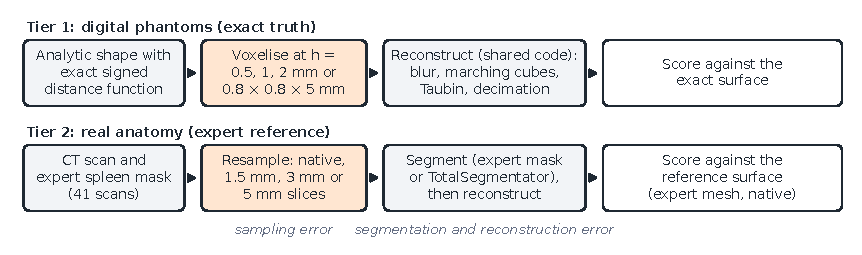
\includegraphics[width=\textwidth]{overview.pdf}
\caption{Study overview. Tier~1 scores reconstructions of analytic phantoms against their exact surfaces. Tier~2 resamples expert-labelled CT before segmentation and scores meshes from the expert mask and from TotalSegmentator against the expert reference surface.}
\label{f:overview}
\end{figure*}

\emph{Tier~1.} Four phantoms with exact signed distance functions covered distinct surface types: a sphere (radius 15\mm), a thin capsule (radius 2\mm, length 44\mm), a torus (radii 18 and 6\mm; genus one) and a rounded box ($28\times20\times12$\mm, 2\mm rounding). Each was placed with a random rotation and sub-voxel offset, voxelised, reconstructed and scored with the exact signed distance function (mesh to truth) and exact point-to-triangle distances (truth to mesh). Exact surfaces measure reconstruction error without a reference of its own, including the error of the canonical procedure that builds the Tier~2 references.

\emph{Tier~2.} Each CT scan and, separately, its expert mask were resampled to each level \emph{before} segmentation. Each coarsened axis was Gaussian filtered with $\sigma_a=(s'_a/s_a-1)/2$ voxels, the anti-aliasing convention of scikit-image~\cite{vanderwalt2014skimage}, then linearly interpolated so that voxel $j$ lies at $j\,s'_a$. All grids thus share one physical frame and need no offset against $S_R$. Resampling the CT, rather than coarsening a finished mask, lets the engine respond to each level as it would to a coarser acquisition; it returned its mask on the same grid. The resampled expert mask, thresholded at 0.5, is a segmentation-free control that isolates sampling error.

\emph{Design.} The design is split-plot~\cite{montgomery2017doe}: whole plots (one segmentation each) are mask source $\times$ resolution level, and sub-plots (one mesh each) are reconstruction settings, crossed in a full factorial grid plus the application's \emph{production} settings.

% ════════════════════════════════════════════════════════════════════════
\section{Data and Experimental Setup}
\emph{Data.} Tier~2 used the 41 training scans of the Medical Segmentation Decathlon Task09 Spleen~\cite{antonelli2022msd} (CC-BY-SA 4.0), each with one expert manual segmentation. In-plane spacing was 0.61--0.98\mm and slice spacing 1.5--8\mm (5\mm in 24 scans). TotalSegmentator was trained on data from one Basel hospital~\cite{wasserthal2023totalsegmentator}, so these scans are external to it, and none was used to tune any setting.

\emph{Factors.} Tier~1 voxelised each phantom at isotropic $h\in\{0.5,1,2\}$\mm and at $0.8\times0.8\times5$\mm, at five placements. Its grid crossed blur $\{0,0.5,1\}$\mm, isosurface variant (Lewiner, Lorensen), Taubin iterations $\{0,10,30,60\}$ and decimation $\{0,0.25,0.5,0.75\}$ (fraction of faces removed): 96 configurations plus production (blur 0.6 voxels, 30 iterations, decimation 0.5), giving 7{,}760 meshes. Tier~2 fixed the isosurface variant, which explained 0.0\% of Tier~1 variance, leaving 48 grid configurations plus production (decimation 0.6 for the engine's masks, as in the application). Its levels were \lvl{native}; \lvl{iso1.5} and \lvl{iso3} (minimum 1.5 and 3\mm on every axis); and \lvl{slice5} (minimum 5\mm slices, native in-plane). \lvl{iso1.5} and \lvl{iso3} resampled all 41 scans and \lvl{slice5} the 14 with thinner slices, giving 16{,}072 meshes.

\emph{Engine.} TotalSegmentator 2.13 in fast mode, the application's default, segmented each resampled scan once; fast mode predicts at 3\mm and returns the mask on the input grid.

\emph{Metrics and statistics.} Each surface was sampled with 20{,}000 points per side; distances were exact point-to-triangle distances (VTK); $\tau=1$\mm. Mask-level Dice compared each mask with the native expert mask after nearest-neighbour mapping to the native grid. Level effects were paired by scan over resampled scans, with 95\% bootstrap confidence intervals over scans (5{,}000 resamples)~\cite{efron1993bootstrap}, Wilcoxon signed-rank tests~\cite{wilcoxon1945} and Holm correction across 12 tests~\cite{holm1979}. Variance shares are descriptive main effects across the tested grid, with 95\% CIs from 1{,}000 bootstrap resamples of scans (Tier~2) or of placements within shape (Tier~1). The $\eta^2$ of scans is the share of the observed sum of squares carried by scan means; a random-intercept model, estimated by ANOVA on the balanced levels (equal to REML for balanced data), instead estimates the variance between scans after removing within-scan noise, so the two differ in estimand and data. The sampling relationship was fitted through the origin, since $\Delta=0$ reproduces the reference exactly. Leave-one-scan-out validation predicted each scan's points from a fit to the other 40 scans and pooled the errors over all 96 points; leave-one-level-out validation predicted each level from a fit to the other two. The grid comparison averaged each scan's 48 configuration-level differences, then averaged over scans with a scan bootstrap CI and a Wilcoxon test. Values are mean $\pm$ SD across scans.

\emph{Implementation.} Python 3.14 (NumPy, SciPy, scikit-image, PyVista/VTK) on a 6-core CPU and an RTX 5080 GPU; seed 2026.

% ════════════════════════════════════════════════════════════════════════
\section{Results}
All 23{,}832 meshes produced a surface, and no mask was empty.

\subsection{Q1: Reconstruction error on exact surfaces}
Spacing dominates reconstruction error. The canonical configuration, which builds the Tier~2 references, has an ASSD of about $0.14\,h$ for every shape (Table~\ref{t:floor}), and placement-to-placement variation is small (coefficient of variation $\leq0.19$).

\begin{table}[!t]
\caption{Tier~1 error floor: ASSD (HD95) in mm of the canonical reconstruction against the exact surface, mean of five placements.}
\label{t:floor}
\centering\footnotesize
\setlength{\tabcolsep}{3pt}
\begin{tabular}{@{}lcccc@{}}
\toprule
Phantom & 0.5\mm & 1\mm & 2\mm & $0.8\times0.8\times5$\mm \\
\midrule
Sphere & 0.070 (0.17) & 0.147 (0.34) & 0.271 (0.75) & 0.495 (1.62) \\
Capsule & 0.069 (0.17) & 0.144 (0.35) & 0.331 (0.77) & 0.634 (1.95) \\
Torus & 0.068 (0.16) & 0.138 (0.33) & 0.278 (0.66) & 0.499 (1.61) \\
Rounded box & 0.072 (0.17) & 0.145 (0.33) & 0.297 (0.68) & 0.525 (1.72) \\
\bottomrule
\end{tabular}
\end{table} Spacing is the largest main effect, with 38.8\% [36.1, 42.0] of ASSD variance against 21.3\% for shape; on the log scale, where its multiplicative interaction with shape largely disappears, it explains 68.6\%. Blur, smoothing, decimation and the isosurface variant together explain 2.2\% (Table~\ref{t:variance}). Smoothing depends on shape: at 2\mm, 30 Taubin iterations reduce ASSD for the sphere (0.309 to 0.199\mm), torus (0.279 to 0.203\mm) and box (0.296 to 0.224\mm) but double it for the capsule (0.425 to 0.844\mm). No mesh is open without decimation (0 of 1{,}920), and at $0.8\times0.8\times5$\mm 64\% of capsule meshes fail the topology check, mostly by splitting into pieces, because 5\mm slices cannot sample a 4\mm tube continuously.

\subsection{Q2: Sampling error on real anatomy}
Coarser acquisition alone moves a correct surface, predictably. Resampling the expert mask moves its canonical surface by 0.204, 0.418 and 0.445\mm at \lvl{iso1.5}, \lvl{iso3} and \lvl{slice5} (Table~\ref{t:tier2}; all $p<0.001$), while Dice stays at 0.985, 0.968 and 0.971. The error follows the added sampling (Fig.~\ref{f:floor}): $\text{ASSD}=0.177\,\Delta$, 95\% CI [0.171, 0.184] from a scan bootstrap, $R^2=0.76$. Predicting each scan from a fit to the other 40 gives $R^2=0.75$ and a mean absolute error of 0.037\mm, so the relationship generalises across scans. Fitted on two levels, it predicts the in-plane levels within 0.028--0.038\mm but slice-only coarsening (\lvl{slice5}) less well (0.109\mm). The coarse grid's geometric-mean or largest spacing does not predict the error ($R^2<0$), because the reference already contains the native sampling. A free intercept gives $0.066+0.145\,\Delta$, whose slope matches Tier~1's $0.14\,h$.

\begin{figure}[!t]
\centering
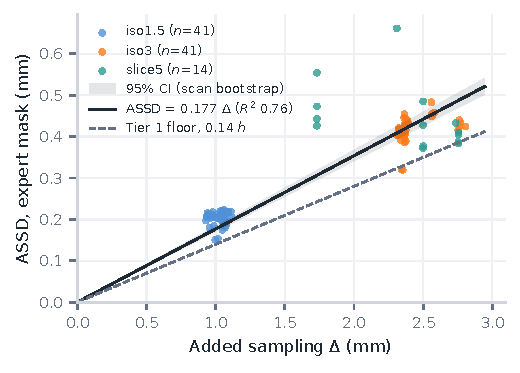
\includegraphics[width=0.92\columnwidth]{sampling_floor.pdf}
\caption{Canonical ASSD of the resampled expert mask against the added sampling $\Delta$ of (\ref{e:delta}): 96 points from 41 scans ($n$ per level in the legend). Solid: fit through the origin, with its 95\% CI from a scan bootstrap (band). Dashed: the Tier~1 floor, $0.14\,h$.}
\label{f:floor}
\end{figure}

\begin{table*}[!t]
\caption{Tier~2 results by resolution level (mean $\pm$ SD across scans; distances in mm; \lvl{slice5}: the 14 resampled scans). Dice is against the native expert mask, ASSD against the reference surface. Change: paired change in canonical ASSD against native [95\% bootstrap CI]; Wilcoxon $p<0.001$ except TotalSegmentator at \lvl{iso1.5} ($p=0.64$) and \lvl{iso3} ($p=0.66$), unchanged by Holm correction. Closed: share of closed meshes.}
\label{t:tier2}
\centering\footnotesize
\setlength{\tabcolsep}{4.5pt}
\begin{tabular}{@{}llrcccccc@{}}
\toprule
 & & & & \multicolumn{2}{c}{Canonical} & \multicolumn{3}{c}{Production} \\
\cmidrule(lr){5-6}\cmidrule(lr){7-9}
Source & Level & $n$ & Dice & ASSD & Change vs native & ASSD & $\bar d_{\pm}$ & Closed \\
\midrule
Expert mask & \lvl{native} & 41 & -- & 0.000 & -- & 0.234 $\pm$ 0.056 & $-0.022$ & 98\% \\
 & \lvl{iso1.5} & 41 & 0.985 $\pm$ 0.003 & 0.204 $\pm$ 0.017 & $+0.204$ [$+0.198$, $+0.209$] & 0.374 $\pm$ 0.098 & $-0.043$ & 95\% \\
 & \lvl{iso3} & 41 & 0.968 $\pm$ 0.006 & 0.418 $\pm$ 0.030 & $+0.418$ [$+0.408$, $+0.426$] & 0.517 $\pm$ 0.126 & $-0.142$ & 98\% \\
 & \lvl{slice5} & 14 & 0.971 $\pm$ 0.011 & 0.445 $\pm$ 0.079 & $+0.445$ [$+0.411$, $+0.490$] & 0.425 $\pm$ 0.127 & $+0.013$ & 93\% \\
\midrule
TotalSegmentator & \lvl{native} & 41 & 0.940 $\pm$ 0.018 & 0.901 $\pm$ 0.197 & -- & 0.948 $\pm$ 0.218 & $+0.221$ & 66\% \\
 & \lvl{iso1.5} & 41 & 0.940 $\pm$ 0.019 & 0.905 $\pm$ 0.223 & $+0.004$ [$-0.019$, $+0.026$] & 0.958 $\pm$ 0.255 & $+0.099$ & 90\% \\
 & \lvl{iso3} & 41 & 0.940 $\pm$ 0.018 & 0.907 $\pm$ 0.206 & $+0.006$ [$-0.006$, $+0.019$] & 0.914 $\pm$ 0.247 & $+0.038$ & 95\% \\
 & \lvl{slice5} & 14 & 0.926 $\pm$ 0.014 & 1.079 $\pm$ 0.152 & $+0.188$ [$+0.150$, $+0.229$] & 1.048 $\pm$ 0.169 & $+0.075$ & 50\% \\
\bottomrule
\end{tabular}
\end{table*}

\subsection{Q3: Automatic segmentation across resolutions}
The engine's error does not depend on in-plane resolution down to 3\mm, rises with thick slices, and is dominated by the patient. Its canonical ASSD is 0.901, 0.905 and 0.907\mm at \lvl{native}, \lvl{iso1.5} and \lvl{iso3}, with both paired confidence intervals containing zero, and its Dice is 0.940 throughout (Table~\ref{t:tier2}, Fig.~\ref{f:assd}). With 5\mm slices its ASSD rises by 0.188\mm and its Dice falls from 0.941 to 0.926 on the same 14 scans. Its error is 2.2--4.4 times that of the resampled expert mask at every coarse level. Patient-to-patient variation explains 89.5\% [65.0, 95.2] of its ASSD variance and resolution 2.7\%, with all reconstruction settings together under 0.5\% (Table~\ref{t:variance}); a random-intercept model assigns 94.2\% of the variance to scans, and the log scale 84.0\%. Its meshes lie outside the expert surface on average ($\bar d_{\pm}=+0.261$\mm canonical at native).

\begin{figure*}[!t]
\centering
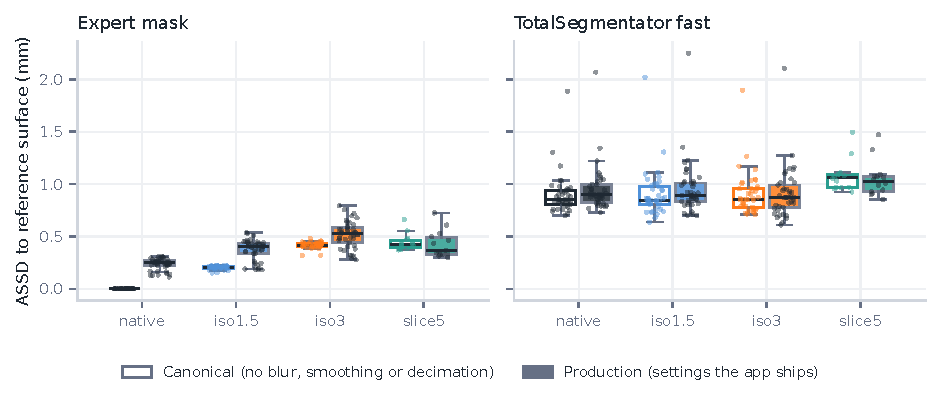
\includegraphics[width=0.76\textwidth]{assd_by_resolution.pdf}
\caption{ASSD to the reference surface by resolution level for the expert mask (left) and TotalSegmentator (right). Hollow boxes: canonical reconstruction; filled: production settings; points: scans.}
\label{f:assd}
\end{figure*}

\begin{table}[!t]
\caption{Descriptive main-effect shares of ASSD variance ($\eta^2$, \%) across the tested grid, with 95\% CIs from a bootstrap over placements within shape (T1) or over scans (T2). TS: TotalSegmentator. T1 interactions + residual include placement replication (2.2\%).}
\label{t:variance}
\centering\scriptsize
\setlength{\tabcolsep}{2.2pt}
% generated by research/paper_stats.py; do not edit by hand
\begin{tabular}{@{}lccc@{}}
\toprule
Factor & T1 phantoms & T2 expert mask & T2 TS \\
\midrule
Spacing / resolution & 38.8 [36.1, 42.0] & 50.5 [47.3, 55.7] & 2.7 [0.2, 15.0] \\
Shape / scan & 21.3 [19.0, 23.5] & 10.3 [6.2, 14.0] & 89.5 [65.0, 95.2] \\
Blur & 0.8 [0.8, 0.9] & 0.9 [0.6, 1.2] & 0.0 [0.0, 0.0] \\
Taubin iterations & 1.2 [1.0, 1.5] & 16.0 [10.4, 23.0] & 0.4 [0.1, 1.4] \\
Decimation & 0.2 [0.2, 0.2] & 0.4 [0.4, 0.5] & 0.0 [0.0, 0.0] \\
Isosurface variant & 0.0 [0.0, 0.0] & -- & -- \\
Interactions + residual & 37.7 [35.6, 39.5] & 21.9 [16.5, 25.5] & 7.4 [2.9, 24.0] \\
\midrule
Scans, random intercept$^{a}$ & -- & 13.0 & 94.2 \\
\bottomrule
\multicolumn{4}{@{}p{0.97\columnwidth}@{}}{\scriptsize $^{a}$Variance between scans in a random-intercept model on the balanced levels (\texttt{native}, \texttt{iso1.5}, \texttt{iso3}): a different estimand from $\eta^2$ (Section~V).}
\end{tabular}

\end{table}

\subsection{Q4: Deployed settings, geometry and topology}

\begin{figure*}[!t]
\centering
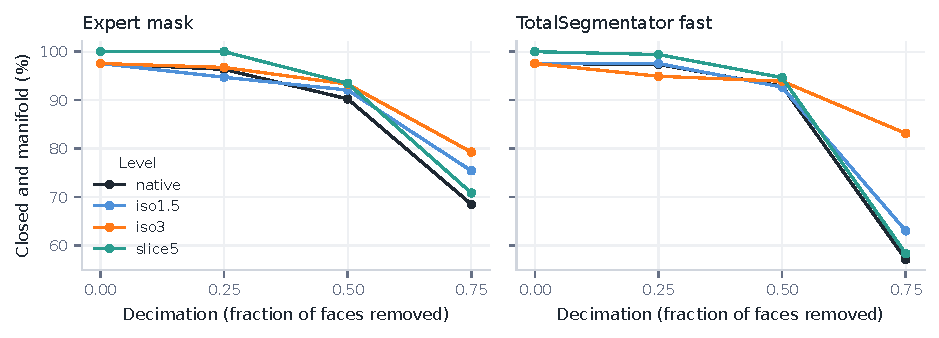
\includegraphics[width=0.68\textwidth]{topology_by_decimation.pdf}
\caption{Share of closed meshes against decimation (fraction of faces removed), by resolution level, for the expert mask (left) and TotalSegmentator (right). One scan cut by the field of view is open at every setting, capping most curves at 98\%.}
\label{f:topology}
\end{figure*}

Production settings shrink thin and coarse-grid structures, and decimation breaks closure without moving unsmoothed geometry. On exact surfaces, production settings reduce the sphere's error at 1\mm (0.147 to 0.088\mm) but raise the 2\mm capsule's from 0.331 to 1.192\mm, shrinking it by 1.13\mm, more than half its radius. On the expert mask they move the surface 0.234\mm at native and 0.517\mm at \lvl{iso3}, where the volume error is $-2.0\%$ (Table~\ref{t:tier2}): the 0.6-voxel blur becomes 1.8\mm on a 3\mm grid.

Decimation explains at most 0.6\% of Tier~2 error variance but drives topology (Fig.~\ref{f:topology}). On the unsmoothed expert mesh it leaves the surface unchanged (ASSD $<10^{-6}$\mm) in 39 of 41 scans at 0.25 and 34 of 41 at 0.5, because decimation first merges the coplanar patches that marching cubes produces; at 0.75 only 57--83\% of meshes stay closed, even in topology-preserving mode. For the engine, production meshes built on the 3\mm grid are both closer to the reference than native-grid meshes ($-0.034$\mm [$-0.055$, $-0.013$], $p=0.003$) and more often closed (95\% against 66\%), with a median of 2{,}600 instead of 19{,}520 faces. Because production blur is set in voxels, this comparison also changes the physical blur. Holding blur in millimetres, smoothing and decimation fixed, the 3\mm grid changes the engine's ASSD by only $-0.017$\mm [$-0.031$, $-0.003$] ($p=0.02$; 27 of 41 scans lower), about 2\% of its error and below the reference floor, but at 0.75 decimation it raises closure from 57\% to 83\% ($+26$ points [20, 32], $p<0.001$; 36 of 41 scans). The grid itself thus improves topology and mesh size, not accuracy. The one scan open at every setting has its spleen cut by the field of view.

% ════════════════════════════════════════════════════════════════════════
\section{Ablation and Sensitivity}

\emph{Unresampled scans.} Counting the 27 scans that \lvl{slice5} left unchanged would dilute its effect on the expert mask from 0.445 to 0.152\mm, so level effects use resampled scans only.

\emph{Numerical reproducibility.} Changing only the crop origin reproduced all 2{,}009 native expert-mask meshes exactly; engine meshes moved by single-precision rounding ($\leq1.5\times10^{-5}$\mm), which decimation amplified to at most 0.016\mm and a closure change in 12 of 1{,}517 meshes (0.8\%).

\emph{Cost.} Tier~1 took 2.8\,min on five CPU workers; Tier~2, 96 GPU engine calls (17--30\,s each) and 28.1\,min of scoring.

% ════════════════════════════════════════════════════════════════════════
\section{Discussion}
\emph{Two regimes.} With a correct segmentation, resolution leads and smoothing follows; with an automatic engine, the patient sets the error and resolution matters only through slice thickness, likely because the fast engine resamples every input to 3\mm. The ranking is thus engine and case, slice thickness, smoothing, then blur and decimation for geometry, while decimation leads for topology.

\emph{The sampling relationship and the tolerance it implies.} Within the tested protocol, $\text{ASSD}\approx0.177\,\Delta$ turns a scan's spacing into an expected error before segmentation. It also bounds the reference: the native reference surface carries about 0.4--0.5\mm of its own sampling error on 5\mm-slice scans and 0.2\mm on slices of 2.5\mm or less, and differences below this floor are departures from the reference staircase, not anatomical error. Smoothing illustrates this: it reduces error for every compact phantom against the truth (Q1), yet moves fine-grid meshes away from the unsmoothed anatomical reference. Surface tolerances should therefore exceed the reference's sampling floor, which rules out a 0.5\mm NSD tolerance on thick-slice data.

\emph{Relation to prior methodology.} Because stages were crossed, the study shows why additive error budgets~\cite{juergensen2024phantom} can mislead: on phantoms about a third of the variance lies in interactions, and smoothing helps or harms depending on shape. The engine's 0.9\mm ASSD is close to the 0.8\mm median segmentation error of the printing literature~\cite{schulze2024qa}, a different statistic, and its degradation at 5\mm but not 3\mm slices matches the cadaver finding~\cite{ahmed2024mandible}.

\emph{Implications.} Report surface metrics alongside Dice, which stayed at or above 0.968 while ASSD rose by up to 0.445\mm; specify blur in millimetres; check closure after decimation where closed meshes are needed, as for printing and volume measurement; and mesh an engine's output on its working grid for closed, compact meshes.

% ════════════════════════════════════════════════════════════════════════
\section{Limitations and Threats to Validity}
\emph{Internal.} Resampling simulates coarser acquisition without kernel, noise or partial-volume differences, so the sampling relationship is probably a lower bound for real acquisitions. The reference inherits native resolution and a single annotator per scan.
\emph{External.} Real-anatomy results cover one compact organ, one dataset and the engine's fast mode; thin structures and finer engines may behave differently, and the 3\mm-grid finding needs confirmation on held-out data.
\emph{Construct.} Global surface metrics can hide local defects, and no task-specific tolerance is evaluated.
\emph{Conclusion.} The $\eta^2$ shares are descriptive main effects of the tested grid, not causal contributions; their CIs resample scans because meshes within a scan are not independent. \lvl{slice5} has 14 scans.

% ════════════════════════════════════════════════════════════════════════
\section{Conclusion}
On exact surfaces, reconstruction error is about $0.14\,h$ and dominated by spacing (Q1). On 41 spleen scans, simulated coarser acquisition alone moves a correct surface by about $0.177\,\Delta$ (Q2). TotalSegmentator's fast-mode error is set mostly by the patient, is unchanged from native to 3\mm grids and rises with 5\mm slices (Q3). Deployed settings shrink thin and coarse-grid structures, decimation breaks closure without moving unsmoothed geometry, and meshing at the engine's working grid improves closure and mesh size, with a negligible change in accuracy (Q4). Methodologically, crossing the stages against an exact and an expert reference reveals interactions that an additive error budget would miss. Future work will add multiple organs, a held-out dataset, real coarse acquisitions and a full-resolution engine, and will predict each case's error without ground truth to select the cheapest pipeline that meets a task's accuracy requirement.

\section*{Data and Code Availability}
\url{https://github.com/Organic42/MEDSYS}, release \texttt{v1.0-paper}: code in \texttt{research/}, per-mesh results in \texttt{research/results/}, paper sources and reproduction commands in \texttt{docs/paper/}. Images: Medical Segmentation Decathlon, CC-BY-SA 4.0~\cite{antonelli2022msd}; not redistributed.

\section*{Acknowledgment}
\todo{Acknowledgements.}

\bibliographystyle{IEEEtran}
\bibliography{references}

\end{document}
